\documentclass[french]{beamer}
\usepackage[utf8]{inputenc}
\usepackage[T1]{fontenc}
\usepackage[french]{babel}
\usepackage{graphicx}
\usetheme{CambridgeUS}
\usecolortheme{beaver}
\useinnertheme{rectangles}

\graphicspath{{./pictures/}}

\definecolor{BlockTitleColor}{rgb}{0.6,0,0}
\definecolor{BlockBodyColor}{rgb}{0.96,0.90,0.90}
\setbeamercolor{block title}{bg=BlockTitleColor,fg=white}
\setbeamercolor{block body}{bg=BlockBodyColor}
\setbeamercolor{titlelike}{bg=BlockTitleColor,fg=white}
\setbeamercolor{frametitle}{bg=BlockTitleColor,fg=white}

\title{RedSquare}
\subtitle{Roguelike en réseau}
\institute[UFC]{Université de Franche-Comté \\ Licence 3}
\author[Lucas G., Rémi S., Vincent T., Florian V.]{Lucas Grosjean \and Rémi Simonin \and Vincent Tourneret \and Florian Vetter}
\begin{document} 

\begin{frame}
\titlepage
\end{frame}

\begin{frame}
\frametitle{Plan de la présentation}
\tableofcontents
\end{frame}

\section{Présentation de RedSquare}

\begin{frame}
\frametitle{Plan}
\tableofcontents[currentsection]
\end{frame}

\begin{frame}
\frametitle{Présentation de RedSquare}
\begin{block}{RedSquare : }
RedSquare est un jeu video produit suivant ces contraintes : 
\begin{itemize}
     \item Utilisation de Gamedev Framework (librairie de développement de jeu 2D en C++)
     \item Jeu de type Roguelike
     \item Jouable en solo et en multijoueur
     \item Utilisation d'une architecture client/serveur
\end{itemize}
\end{block}
\end{frame}

\begin{frame}
\frametitle{Présentation de RedSquare}
\begin{block}{Définition (Roguelike) }
Le Roguelike est un genre de jeu vidéo où :
\begin{itemize}
    \item Le joueur évolue dans un donjon pleins de récompenses
    \item Le donjon est généré procéduralement
    \item Le jeu se joue en tour par tour
    \item Le joueur se bat contre des monstres
    \item La mort est définitive
\end{itemize}
\end{block}
\end{frame}

\section{Modélisation}

\subsection{Relation serveur/client}

\begin{frame}
\frametitle{Plan}
\tableofcontents[currentsection,currentsubsection]
\end{frame}

\begin{frame}
\frametitle{Réseau}
\begin{columns}
    \begin{column}{0.34\textwidth}
        \begin{itemize} 
            \item Le serveur est autoritaire. %% Définition de autoritaire ?
            \item Utilisation de gf::net pour l'application des protocoles.
        \end{itemize}
    \end{column}
    \begin{column}{0.66\textwidth}
        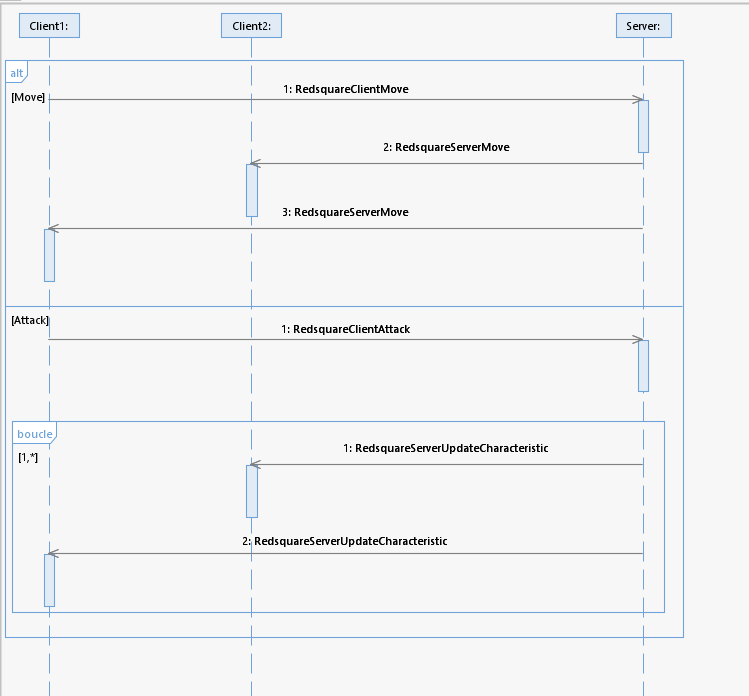
\includegraphics[scale=0.3]{./Diagramme/Deplacement}
    \end{column}
\end{columns}
\end{frame}

\subsection{Gamedev Framework}

\begin{frame}
\tableofcontents[currentsection,currentsubsection]
\end{frame}

\begin{frame}
\frametitle{Gamedev Framework}
\begin{block}{Fonctionnalités de GF utilisées dans notre projet}
\begin{itemize}
    \item Structure de données unique (Vector2i, SquareMap)
    \item Id (Identifiant de chaque entité du jeu)
    \item Fonction de rendu graphique
    \item Serialization (Pour la communication client/serveur)
    \item Gf Net pour les protocoles
    \item Scene (Transition entre menu/jeu)
    \item Widget
\end{itemize}
\end{block}
\end{frame}


\section{Implémentation}

\subsection{Génération procédurale}

\begin{frame}
\frametitle{Plan}
\tableofcontents[currentsection,currentsubsection]
\end{frame}

\begin{frame}
\frametitle{Génération procédurale}

\only<1>{
    \begin{block}{Définition (Génération procédurale) }
    La génération procédurale est une manière de générer du contenu numérique de manière automatisé en s'appuyant sur des algorithmes.
    \end{block}
}
\only<2>{
    \center
    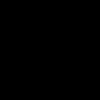
\includegraphics[width=10cm,height=6cm]{./Procedural/void}
}
\only<3>{
    \center
    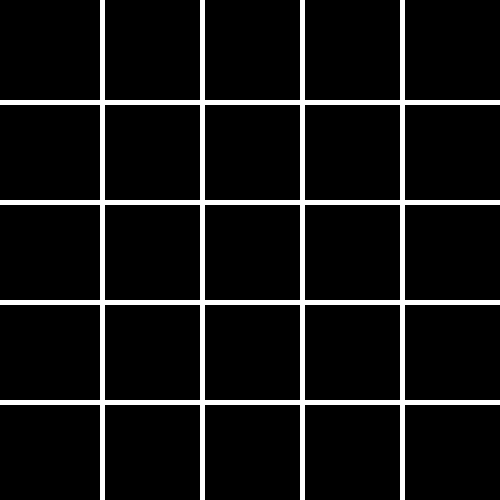
\includegraphics[width=10cm,height=6cm]{./Procedural/grid}
}
\only<4>{
    \center
    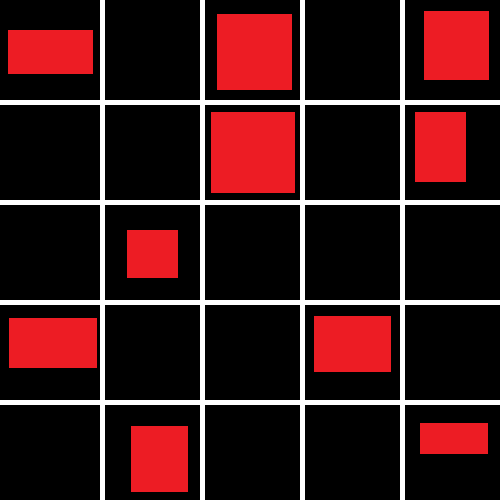
\includegraphics[width=10cm,height=6cm]{./Procedural/floor}
}
\only<5>{
    \center
    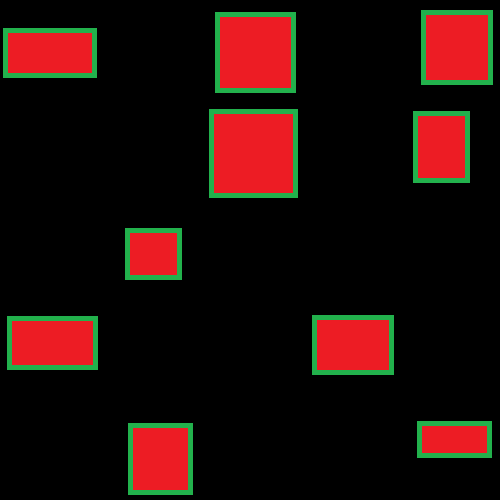
\includegraphics[width=10cm,height=6cm]{./Procedural/wall}
}
\only<6>{
    \center
    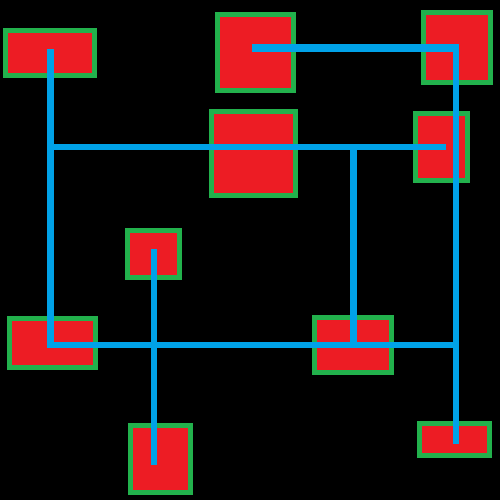
\includegraphics[width=10cm,height=6cm]{./Procedural/corridor}
}
\only<7>{
    \center
    
\includegraphics[width=10cm,height=6cm]{./Procedural/stair}
}
\end{frame}


\begin{frame}
\frametitle{Image du jeu}     
\center
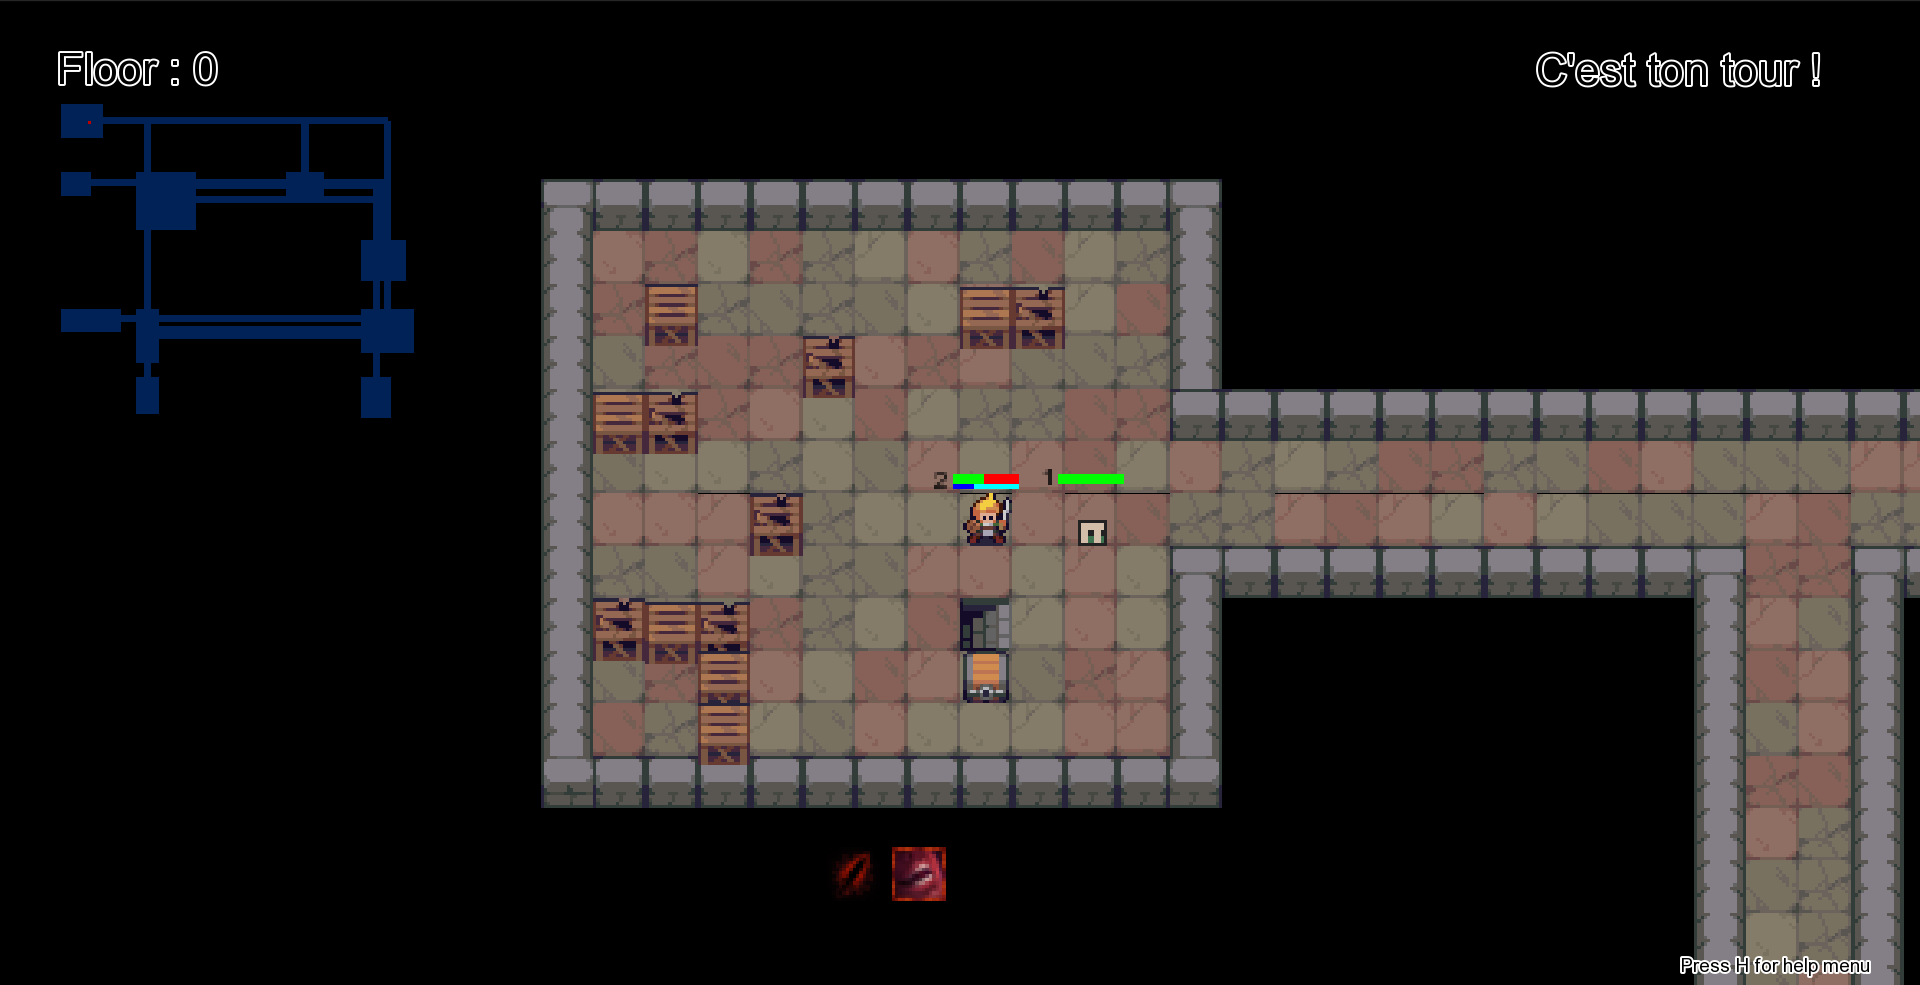
\includegraphics[scale=0.15]{Apercu_jeu}
\end{frame}

\begin{frame}
\frametitle{Salle de boss}
\begin{block}{Salle de boss : }
Ces salles ajoutent de la diffculté au jeu :
\begin{itemize}
\item Génération manuelle donc facilement personnalisable
\item Facile à produire
\item Remplies d'ennemies
\item Pleines de récompenses
\item Apparition périodique
\end{itemize}
\end{block}

\begin{block}{Implémentation: }
Parcours d'un tableau de caractère où chaque symbole corrrespond à un case spéciale.\\ 
\end{block}

\end{frame}

\begin{frame}
\frametitle{Salle de boss}
\begin{tabular}{  c  c  }
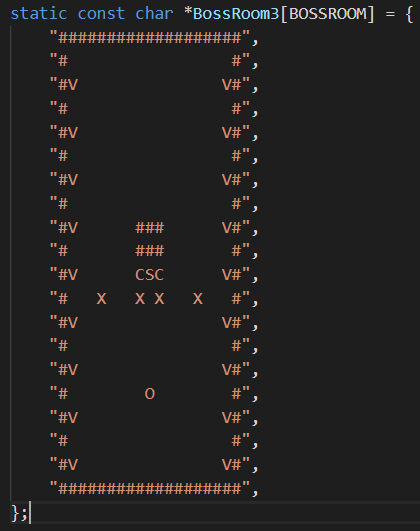
\includegraphics[scale=0.6]{./BossRoom}
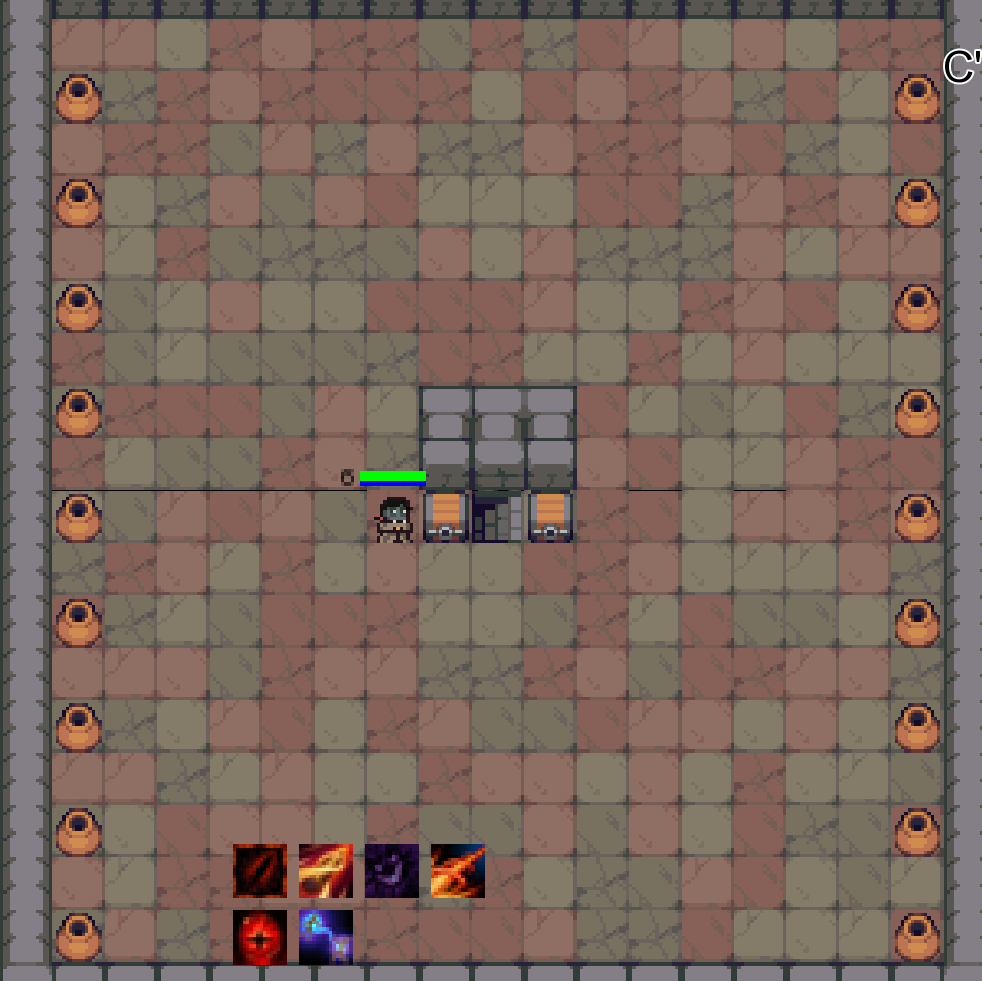
\includegraphics[scale=0.19]{./Salle_Boss}
\end{tabular}
\end{frame}

\subsection{Sorts}

\begin{frame}
\frametitle{Plan}
\tableofcontents[currentsection,currentsubsection]
\end{frame}

\begin{frame}
\frametitle{Sorts}
\begin{block}{Hiérarchie de classe}
L'utilisation d'un seule classe permet d'optimiser le traitement à la création et facilite l'utilisation dans les structures de données.
\end{block}

\begin{block}{Gestion des sorts}
\begin{itemize}
    \item 1) Envoie d'un paquet du client au serveur.
    \item 2) Traitement du serveur avec la bonnes méthodes.
    \item 3) Renvoi d'un paquet aux clients avec les nouvelles données.
\end{itemize}
\end{block}

\end{frame}

\subsection{Objets}

\begin{frame}
\frametitle{Plan}
\tableofcontents[currentsection,currentsubsection]
\end{frame}

\begin{frame}
\frametitle{Objets}

\begin{block}{Hiérarchie de classe :}
L'utilisation d'un seule classe permet d'optimiser le traitement à la création et facilite l'utilisation dans les structures de données.
\end{block}

\begin{block}{Type d'objet}
Un objet est soit un équipement, soit un consommable.
\end{block}

\begin{block}{Gestion des objets} 
\begin{itemize}
\item Equipement : Envoie d'un paquet du serveur contenant les nouvelles caractéristiques du joueurs à tous les joueurs.
\item Consommable : Envoie d'un paquet au serveur contenant le sous-type de l'objet et le serveur éxécute la méthode associé à l'objet, puis renvoie des nouvelles données à tous les clients.
\end{itemize}
\end{block}

\end{frame}

\begin{frame}
\frametitle{Inventaire}
\begin{columns}
    \begin{column}{0.34\textwidth}
    
        \begin{block}{Implémentation}
         L'inventaire est une map dont la clé est un entier corrrespondant à la position du slot dans l'inventaire est dont la valeur est un item (nullptr si vide)
        \end{block}
        \begin{block}{Gestion graphique}
            Utilisation de widgets pour afficher l'inventaire.\\
            Placement manuelle des slots de l'inventaire.\\
        \end{block}
        
    \end{column}
    \begin{column}{0.66\textwidth}
    
    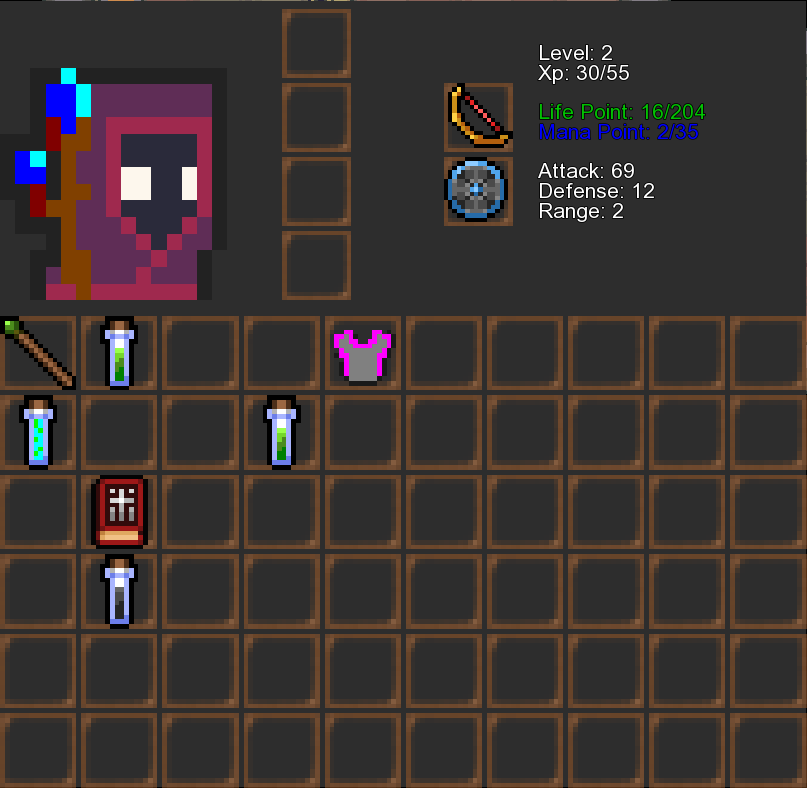
\includegraphics[scale=0.25]{Inventaire}
    
    \end{column}
\end{columns}
\end{frame}

\begin{frame}
\frametitle{Inventaire}

\begin{block}{Caractéristiques}
Les caractéristiques du joueur sont donnée par le serveur puis affiché sur l'inventaire     
\end{block}

\begin{block}{Déplacement}
\begin{itemize}
    \item 1) Envoie d'un paquet au serveur avec la position actuelle et la position voulu. 
    \item 2) Le serveur déplace l'objet si il n'y à rien à cette position sinon il permute les 2 objets.
    \item 3) Renvoie d'un paquet au client pour renseigner le changement de position
\end{itemize}
\end{block}
\end{frame}

\begin{frame}
\frametitle{Potions}

\begin{block}{Type de potion} 
\begin{tabular}{  | c | c | c |}
    \hline
    Potion de vie & Potion de mana & Potion d'énergie (vie + mana)\\
    \hline
    Boost de vie & Boost de mana & Boost d'attaque\\
    \hline
    Boost de défense & Boost d'expérience &\\
    \hline
\end{tabular}
\end{block}
\begin{block}{Tier de potion} 
Tous les tiers ne sont pas accesible depuis le début : 
\begin{itemize}
     \item Tier 1 : Tout le jeu (25\% pour les potions, +2 pour les boosts )
     \item Tier 2 : 6ème étage (50\% pour les potions, +5 pour les boosts )
     \item Tier 3 : 16ème étage (70\% pour les potions, +10 pour les boosts)
\end{itemize}
\end{block}
\end{frame}


\begin{frame}
\frametitle{Equipements}

\begin{columns}
    \begin{column}{0.34\textwidth}
    
        \begin{block}{Implémentation}
        Il existe 15 type de chaque équipement, chacun possède des caractéristiques différentes.\\ 
        \end{block}
        
        \begin{block}{Caractéristiques}
            Elles sont calculés à l'appartition de ses objets en multipliant un ratio (différents par type d'objets) par le numéro de l'étage courant.
        \end{block}
    \end{column}
    \begin{column}{0.66\textwidth}
    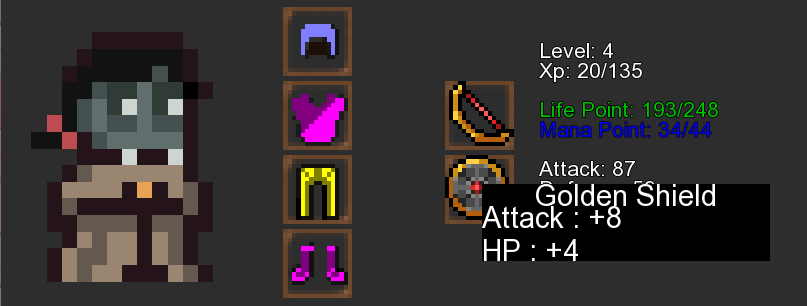
\includegraphics[scale=0.28]{Equipements}
    \end{column}
\end{columns}
\end{frame}

\begin{frame}
\frametitle{Coffre}
\begin{block}{Génération}
Chaque pièce de la carte à 33\% de contenir un coffre.    \\
Un coffre est considéré comme un prop, au contraire que celui ci est associé à un inventaire (identique au joueur).
\end{block}

\begin{block}{Implémentation} 
A l'apparition d'un coffre, on le rempli de 1 à N-1 potion(s) (où N est le numéro de l'étage courant), et d'1 pièce d'équipement.\\
Tous les objets ont la même chance d'apparaitre dans un coffre.
\end{block}
\end{frame}


\begin{frame}
\frametitle{Mini-Map}
   
\begin{block}{Implémentation}
Nous effectuons un parcours sur le tableau de jeu en transformant le type de la case en un pixel de couleur.\\
Nous rendons ensuite cette Mini-Map sur l'écran du joueur, celle-ci est mis-à-jour à chaque déplacement du joueur pour rendre sa position.
\end{block}

\center
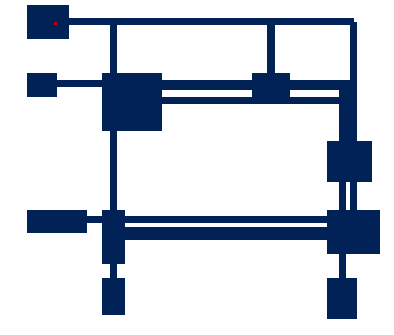
\includegraphics[scale=0.5]{Mini-Map}

\end{frame}

\subsection{Déroulement du jeu}

\begin{frame}
\frametitle{Plan}
\tableofcontents[currentsection,currentsubsection]
\end{frame}

\begin{frame}
\frametitle{Déplacement des entités}
\begin{block}{Déplacement des ennemis}
A L'apparition des monstres, le serveur tire un point sur la carte où celui ci se dirige, une fois à cette position, le serveur tire une nouvelle position.\\ 
Ce cycle continu jusqu'à ce qu'un joueur rentre dans le champ de vision du monstre (7 cases)
\end{block}
\begin{block}{Déplacement des joueurs}
Les joueurs peuvents se déplacer grâce aux fleches directionelles ou avec ZQSD, il se dirige donc case par case.\\
Ils ont aussi la possibilité de se déplacer à la souris en sélectionnant la position d'arrivée voulu, le serveur effectura les déplacements nécéssaire jusqu'à ce point en passant les tours automatiquement.
\end{block}
\end{frame}


\section{Organisation de travail}

\begin{frame}
\frametitle{Plan}
\tableofcontents[currentsection]
\end{frame}

\begin{frame}
\frametitle{Relation intra-groupes}

\begin{block}{Coworking}
Journée de travail tous ensemble pour avancer efficacement.
\end{block}

\begin{block}{Seul}
Développement chacun de son coté sur des fonctionnalités du jeu.
\end{block}
\begin{block}{Pair programming}
Technique de programmation par paire pour les développements plus complexes.
\end{block}
\end{frame}


\begin{frame}
\frametitle{Relation groupe-tuteur}

\begin{block}{Réunion avec notre tuteur}
Bilan sur l'avancé du projet, sur les prochains objectifs à atteindre, réponses à nos questions sur l'implémentation.
\end{block}

\begin{block}{Gamedev Framework}
Collaboration entre notre groupe et notre tuteur pour étoffer l'étendue de la librairie.
\end{block}

\begin{block}{Dead Pixels Society}
Club de développement de jeux vidéo où l'on venait pour interagir avec notre encadrants.
\end{block}
\end{frame}


\begin{frame}
\frametitle{Limites techniques}
Performance réseau faible \\
Son \\
Animation \\
Equilibrage \\
Dette technique (faible mais présente)
\end{frame}

\end{document}